% \documentclass[9pt,t]{beamer}
\usefonttheme{professionalfonts}
\usefonttheme{serif}
\PassOptionsToPackage{pdfpagemode=FullScreen}{hyperref}
\PassOptionsToPackage{usenames,dvipsnames}{color}
\DeclareGraphicsRule{*}{mps}{*}{}
\usepackage{linalgjh}
\usepackage{present}
\usepackage{directories}  % define \grdir, etc.
\usepackage{xr}\externaldocument{\grdir gr2} % read refs from .aux file
\usepackage{catchfilebetweentags}
\usepackage{etoolbox} % from http://tex.stackexchange.com/questions/40699/input-only-part-of-a-file-using-catchfilebetweentags-package
\makeatletter
\patchcmd{\CatchFBT@Fin@l}{\endlinechar\m@ne}{}
  {}{\typeout{Unsuccessful patch!}}
\makeatother

\mode<presentation>
{
  \usetheme{boxes}
  \setbeamercovered{invisible}
  \setbeamertemplate{navigation symbols}{} 
}
\addheadbox{filler}{\ }  % create extra space at top of slide 
\hypersetup{colorlinks=true,linkcolor=blue} 

\title[Linear Geometry] % (optional, use only with long paper titles)
{One.II Linear Geometry}

\author{\textit{Linear Algebra} edition four \\ {\small Jim Hef{}feron}}
\institute{
  \texttt{https://hefferon.net/linearalgebra} \\[0.25ex]
  \texttt{http://joshua.smcvt.edu/linearalgebra}
}
\date{}


\subject{Linear Geometry}
% This is only inserted into the PDF information catalog. Can be left
% out. 

\begin{document}
\begin{frame}
  \titlepage
\end{frame}

% =============================================
\begin{frame}{Geometry} 
We can draw two-unknown equations as lines.
Then the three possibilities for solution sets become clear.
\pause
\begin{center} % had to copy because the graphics are in a different dir
  \begin{minipage}[b]{1.35in}
    \raisebox{-2pt}[8pt][0pt]{\small \begin{tabular}{@{}l}
      \small \textit{Unique solution}
    \end{tabular}}
    \begin{center}
      \includegraphics{\grmpdir ch1.3} \\[.75ex]
      \small $\begin{linsys}{2}
                         3x  &+  &2y  &=  &7   \\
                         x   &-  &y   &=  &-1
                       \end{linsys}$
    \end{center}
  \end{minipage}
  \hspace*{0em}
  \begin{minipage}[b]{1.35in}
    \raisebox{-2pt}[8pt][0pt]{\small \begin{tabular}{@{}l}
      \small \textit{No solutions}
    \end{tabular}}
    \begin{center}
      \includegraphics{\grmpdir ch1.4} \\[.75ex]
      \small $\begin{linsys}{2}
                         3x  &+  &2y  &=  &7   \\
                         3x  &+  &2y  &=  &4
                       \end{linsys}$
    \end{center}
  \end{minipage}
  \hspace*{0em}
  \begin{minipage}[b]{1.35in}
    \raisebox{-2pt}[8pt][0pt]{\small \begin{tabular}[t]{@{}l}
      \textit{Infinitely many} \\
      \textit{solutions}
    \end{tabular}}
    \begin{center}
      \includegraphics{\grmpdir ch1.5}         \\[.75ex]
      \small $ \begin{linsys}{2}
                         3x  &+  &2y  &=  &7   \\
                         6x  &+  &4y  &=  &14
                       \end{linsys}$
    \end{center}
  \end{minipage}
\end{center}
This is a nice restatement of the possibilities; 
the geometry gives us insight into what can happen with linear systems.
\end{frame}



% ..... One.II.1 .....
\section{Vectors in space}
\begin{frame}{Vectors}
A \definend{vector} is an object consisting of a magnitude and a direction.
\centergraphic{\grmpdir ch1.8}
A vector can model a displacement.

\pause
Two vectors with the same magnitude and
same direction, such as all of these, are equal.  
\centergraphic{\grmpdir ch1.12}
For instance, each of the 
above could model a displacement of one over and two up.
\end{frame}




% ..........
\begin{frame}
Denote the vector that extends from $(a_1,a_2)$ to $(b_1,b_2)$ by
\begin{equation*}
  \colvec{b_1-a_1 \\ b_2-a_2}
\end{equation*}
so the ``one over, two up'' vector would be written in this way.
\begin{equation*}
  \colvec{1 \\ 2}
\end{equation*}
\pause
We often picture a vector
\begin{equation*}
  \vec{v}=\colvec{v_1 \\ v_2}
\end{equation*}
as starting at the origin.
From there $\vec{v}$ extends to $(v_1,v_2)$ and we may refer to it
as ``the point $\vec{v}\,$''
so that we may call each of these $\Re^2$.
\begin{equation*}  
   \set{(x_1,x_2)\suchthat x_1,x_2\in\Re}
   \qquad
   \set{\colvec{x_1 \\ x_2}\suchthat x_1,x_2\in\Re}
\end{equation*}
\end{frame}




% ..........
\begin{frame}
These definitions extend to higher dimensions.
The vector that
starts at \( (a_1,\ldots,a_n) \) and ends at \( (b_1,\ldots,b_n) \) 
is represented by this column
\begin{equation*}
  \colvec{b_1-a_1 \\ \vdotswithin{b_1-a_1} \\ b_n-a_n}
\end{equation*}
and two vectors are equal if they have the same representation.
Also, 
we aren't too careful about distinguishing between a point and the vector 
which, when it starts at the origin, ends at that point. 
\begin{equation*}
  \Re^n=
  \set{\colvec{v_1 \\ \vdotswithin{v_1} \\ v_n}\suchthat v_1,\ldots,v_n\in\Re}
\end{equation*}
\end{frame}



% ..........
\begin{frame}{Vector operations}
Scalar multiplication makes a vector longer or shorter, 
including possibly flipping it around.
\centergraphic{\grmpdir ch1.13}
\pause
Where \( \vec{v} \) and \( \vec{w} \) represent displacements,
the vector sum \( \vec{v}+\vec{w}\/ \) represents those displacements combined.
\begin{center}
\includegraphics{\grmpdir ch1.14}
\qquad
\includegraphics{\grmpdir ch1.15}
\end{center}
The second drawing shows the \definend{parallelogram rule} for vector addition.
\end{frame}



% ..........
\begin{frame}{Lines}
The line in $\Re^2$ through \( (1,2) \) and \( (3,1) \)
is comprised of the vectors in this set
\begin{center}
  {$\displaystyle   
     \set{ \colvec[r]{1 \\ 2}+t\colvec[r]{2 \\ -1}\suchthat t\in\Re}
  $}
  \qquad
  \vcenteredhbox{\includegraphics{\grmpdir ch1.16}}
\end{center}
(that is, it is comprised of the endpoints of those vectors).
\pause
% That description expresses this picture.
% \centergraphic{\grmpdir ch1.16}
The vector associated with the parameter \( t \)
\begin{equation*}
  \colvec[r]{2 \\ -1}
\end{equation*}
is a \definend{direction vector}\index{vector!direction}%
\index{direction vector} for the line.
Lines in higher dimensions work the same way.
\end{frame}



% ..........
\begin{frame}{Planes}
The plane in $\Re^3$ through the points
\( (1,0,5) \), \( (2,1,-3) \), and \( (-2,4,0.5) \) consists of
(endpoints of) the vectors in this set.
\begin{center}
  $\set{ \colvec[r]{1 \\ 0 \\ 5}
         +t\colvec[r]{1 \\ 1 \\ -8}
         +s\colvec[r]{-3 \\ 4 \\ -4.5}
       \suchthat t,s\in\Re      }$
  \qquad
  \vcenteredhbox{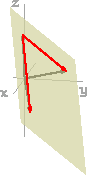
\includegraphics{asy/one_ii_plane.pdf}}
\end{center}
The column vectors associated with a parameter, shown here in red,
\begin{equation*}
  \colvec[r]{1 \\ 1 \\ -8}
  =
  \colvec[r]{2 \\ 1 \\ -3}
  -
  \colvec[r]{1 \\ 0 \\ 5}
  \qquad
  \colvec[r]{-3 \\ 4 \\ -4.5}
  =
  \colvec[r]{-2 \\ 4 \\ 0.5}
  -
  \colvec[r]{1 \\ 0 \\ 5}
\end{equation*}
have their whole body in the plane, not just their endpoint.
% \end{frame}


% \begin{frame}
A set of the form
$\set{\vec{p}+t_1\vec{v}_1+t_2\vec{v}_2+\cdots+t_k\vec{v}_k
             \suchthat t_1,\ldots ,t_k\in\Re}$
where \( \vec{v}_1,\ldots,\vec{v}_k\in\Re^n \) 
and $k\leq n$ is a
\definend{\( k \)-dimensional linear surface}\index{linear surface}
(or \definend{\( k \)-flat}\index{flat}).
\end{frame}




% ..... One.II.2 .....
\section{Length and angle measures}
\begin{frame}{Length} 
\df[df:Length]
\ExecuteMetaData[\grdir gr2.tex]{df:Length}
\ex
The length of
\begin{equation*}
  \vec{v}=\colvec[r]{-1 \\ -2 \\-3}
\end{equation*}
is $\absval{\vec{v}}=\sqrt{1+4+9}=\sqrt{14}$.

\pause
For any nonzero vector $\vec{v}$, the length one vector with the same direction
is $\vec{v}/\absval{\vec{v}}$.
We say that this
\definend{normalizes}\index{normalize}\index{vector!normalize}
$\vec{v}$ to unit length. 
\begin{equation*}
  \frac{\vec{v}}{\absval{\vec{v}}}=\colvec[r]{-1/\sqrt{14} \\ -2/\sqrt{14} \\-3/\sqrt{14}}
\end{equation*}
Note that $\sqrt{(-1/\sqrt{14})^2+(-2/\sqrt{14})^2+(-3/\sqrt{14})^2}$ 
equals~$1$.
\end{frame}




% ..........
\begin{frame}{Dot product} 
\df[df:DotProduct]
\ExecuteMetaData[\grdir gr2.tex]{df:DotProduct}

\ex
The dot product of two vectors
\begin{equation*}
  \colvec{1 \\ 1 \\ -1}\dotprod\colvec{3 \\ -3 \\ 4}
  =3-3-4=-4
\end{equation*}
is a scalar, not a vector.

\pause
The dot product of a vector with itself 
$\vec{v}\dotprod\vec{v}=v_1^2+\cdots+v_n^2$
is the square of the vector's length.
\end{frame}




% ..........
\begin{frame}{Triangle Inequality} 
\th[th:TriangleInequality]
\ExecuteMetaData[\grdir gr2.tex]{th:TriangleInequality}

This is the source of the familiar saying, 
``The shortest distance between two points is in a straight line.''
\centergraphic{\grmpdir ch1.23}
\end{frame}




% ..........
\begin{frame}
\pf[th:TriangleInequality]
\ExecuteMetaData[\grdir gr2.tex]{pf:TriangleInequality0}

\pause
\ExecuteMetaData[\grdir gr2.tex]{pf:TriangleInequality1}
\end{frame}




% ..........
\begin{frame}
\ExecuteMetaData[\grdir gr2.tex]{pf:TriangleInequality2}
\qed
\end{frame}




% ..........
\begin{frame}{Cauchy-Schwarz Inequality} 
\co[th:CauchySchwarz]
\ExecuteMetaData[\grdir gr2.tex]{co:CauchySchwarzInequality}
\pause
\pf[th:CauchySchwarz]
\ExecuteMetaData[\grdir gr2.tex]{pf:CauchySchwarzInequality}
\end{frame}




% ..........
\begin{frame}{Angle measure} 
\df
The \definend{angle} between two vectors $\vec{u},\vec{v}\in\Re^n$
is this.
\begin{equation*}
  \theta
  =
  \arccos(\,\frac{\vec{u}\dotprod\vec{v}}{
         \absval{\vec{u}\,}\,\absval{\vec{v}\,} }\,)
\end{equation*}

We motivate that definition with
two vectors in \( \Re^3 \). 
\centergraphic{\grmpdir ch1.21}
If neither is a multiple of the other then they determine a plane, because if
we put them in canonical position then the origin and the endpoints
make three noncolinear points. 
Consider the triangle formed by
\( \vec{u} \), \( \vec{v} \), and \( \vec{u}-\vec{v} \).
\end{frame}\begin{frame}
\centergraphic{\grmpdir ch1.22}
Apply the Law of Cosines:
$\absval{\vec{u}-\vec{v}\,}^2
  =
  \absval{\vec{u}\,}^2+\absval{\vec{v}\,}^2-
    2\,\absval{\vec{u}\,}\,\absval{\vec{v}\,}\cos\theta$ 
where \( \theta \) is the angle that we want to find.
The left side gives 
\begin{multline*}
(u_1-v_1)^2+(u_2-v_2)^2+(u_3-v_3)^2  \\
     =(u_1^2-2u_1v_1+v_1^2)+(u_2^2-2u_2v_2+v_2^2)+(u_3^2-2u_3v_3+v_3^2)
\end{multline*}
while the right side gives this.
\begin{equation*}
(u_1^2+u_2^2+u_3^2)+(v_1^2+v_2^2+v_3^2)-
     2\,\absval{\vec{u}\,}\,\absval{\vec{v}\,}\cos\theta
\end{equation*}
Canceling squares $u_1^2$ \ldots{}, $v_3^2$ and dividing by $2$ gives 
the formula.
\end{frame}




% ..........
\begin{frame}
\co[co:VectorsOrthogonalIffDoTProductZero]
\ExecuteMetaData[\grdir gr2.tex]{co:VectorsOrthogonalIffDoTProductZero}
\end{frame}




%...........................
% \begin{frame}
% 
% \end{frame}
\end{document}
